% Current evidence-aligned short draft, 2026-09-24.
% Legacy filename only; not submitted and not certified four-page/venue compliant.
% No venue style is assumed installed. Compile from paper/ after installing a TeX engine.
\documentclass[10pt]{article}
\usepackage[margin=1in]{geometry}
\usepackage[T1]{fontenc}
\usepackage{amsmath,amssymb,booktabs,graphicx}
\usepackage[hidelinks]{hyperref}
\title{Better Projection and Stable Fitting Do Not Guarantee Generalization in DeepONet}
\author{Author information to be supplied}
\date{Research draft, September 24, 2026}
\begin{document}
\maketitle
\begin{abstract}
We examine whether offline basis quality and training convergence predict better
operator generalization in a supervised PDEBench Burgers case study. Zero-residual
initialization improves final validation in 29 of 30 paired comparisons.
For 128 training functions, cosine decay produces stable projection-level fitting
in all 20 decay runs; constant learning rates do so in zero of ten small-batch and
one of ten full-batch runs. Nonetheless, small-batch decay worsens validation error
in every seed of both trunk families, also under RMSE. The evidence separates
representation, sampled convergence and generalization within this protocol;
it does not establish a new optimizer, universal mechanism or state-of-the-art method.
\end{abstract}

\section{Scope and related work}
Two-step training and orthonormalization precede our study \cite{lee2023}.
Learned physics-informed DeepONet bases have also been analyzed \cite{williams2024}.
POD-DeepONet is a necessary future reference \cite{lu2022}.
Zero residual mechanisms \cite{rezero} and scheduling techniques \cite{sgdr} are not
new contributions. Generalization issues associated with larger batches are also
established \cite{keskar}; no sharpness mechanism is demonstrated here.
Our public-data experiments use supervised values, not a physics loss.

\section{Projection diagnostic}
Let $S,Y\in\mathbb{R}^{N\times m}$ be target and prediction matrices on the same
points and functions, $L$ a known affine offset, and $P=QQ^\top$ the orthogonal
projector onto a retained numerical feature space. The oracle is $L+P(S-L)$.
If $Y-L$ is in that space, then
\[
 \|S-Y\|_F^2=\|(I-P)(S-L)\|_F^2+
             \|P(S-L)-(Y-L)\|_F^2.
\]
All terms can be normalized by $\|S\|_F^2$. This standard squared-error identity
does not imply that subtracting mean relative $L^2$ values isolates optimization.
The in-space term can involve capacity, fitting and generalization. The oracle
uses target labels with independent sample coefficients and is not a predictive model.
Numerical rank, bias relaxation and outside-span residuals must be stated.

\section{Protocol}
We use a fixed PDEBench Burgers subset \cite{pdebench}, mapping $t=0$ to $t=1$
on 256 subsampled points, with 1000/200/200 training/validation/test functions.
Five seeds share the data partition. Initial MLP/Fourier DeepONet and FNO comparisons
use 1500 updates. Later frozen-trunk interventions use 3000 branch updates.
Trunks and normalization already saw the original 1000 training functions;
small-subset fitting is not few-shot learning.

Four sequential families contain 15, 40, 60 and 40 run records.
Ten stability controls exactly reproduce earlier controls, not independent replicates.
For the stability factorial, all models use zero residual initialization, 128 training
functions, Adam, and either constant $10^{-3}$ or cosine decay to $10^{-5}$, with batch
32 or 128. We evaluate the prescribed final checkpoint. Stability requires excess
relative Frobenius error $\leq0.01$ at all four logged steps
2250/2500/2750/3000. Full batches process four times as many examples per update.

\section{Results}
Initial test mean relative $L^2$ is 0.39357 for MLP DeepONet, 0.41231 for Fourier
DeepONet and 0.22835 for FNO; the input-mean baseline is 0.37577.
Fourier has a better projection fit without better predictions. Conditioning alone
does not beat the baseline. Zero initialization helps validation in 29/30 pairs
and achieves the final fitting threshold in all ten $n=32$ runs, but not reliably
at $n=128$ or $n=1000$ under constant learning rates.

\begin{table}[ht]
\centering\small
\begin{tabular}{lllrrr}
\toprule
Trunk & LR & Batch & Train excess & Stable & Validation rel.\ $L^2$\\
\midrule
MLP & constant & 32 & 0.034534 & 0/5 & 0.44657\\
MLP & constant & 128 & 0.004113 & 0/5 & 0.50846\\
MLP & cosine & 32 & 0.001117 & 5/5 & 0.45708\\
MLP & cosine & 128 & 0.000061 & 5/5 & 0.47377\\
Fourier & constant & 32 & 0.030453 & 0/5 & 0.55232\\
Fourier & constant & 128 & 0.008727 & 1/5 & 0.56900\\
Fourier & cosine & 32 & 0.005602 & 5/5 & 0.58755\\
Fourier & cosine & 128 & 0.000809 & 5/5 & 0.59345\\
\bottomrule
\end{tabular}
\caption{Five-seed means, zero initialization, $n=128$. Stable means all four final
logged points fit to within the projection-excess threshold. Complete seed standard
deviations and per-seed results are in the full manuscript and result summaries.}
\end{table}

Cosine stabilizes fitting in 20/20 runs. Constant full-batch training reaches the
threshold and rebounds in every seed. At batch 32, decay worsens validation in
all five seeds of each trunk; RMSE also increases, from 0.171690 to 0.176732 (MLP)
and from 0.201126 to 0.216168 (Fourier).
MLP full-batch decay improves validation over constant full-batch, so deterioration
is not universal. No group beats the validation input-mean baseline 0.374509.

\begin{figure}[ht]
\centering
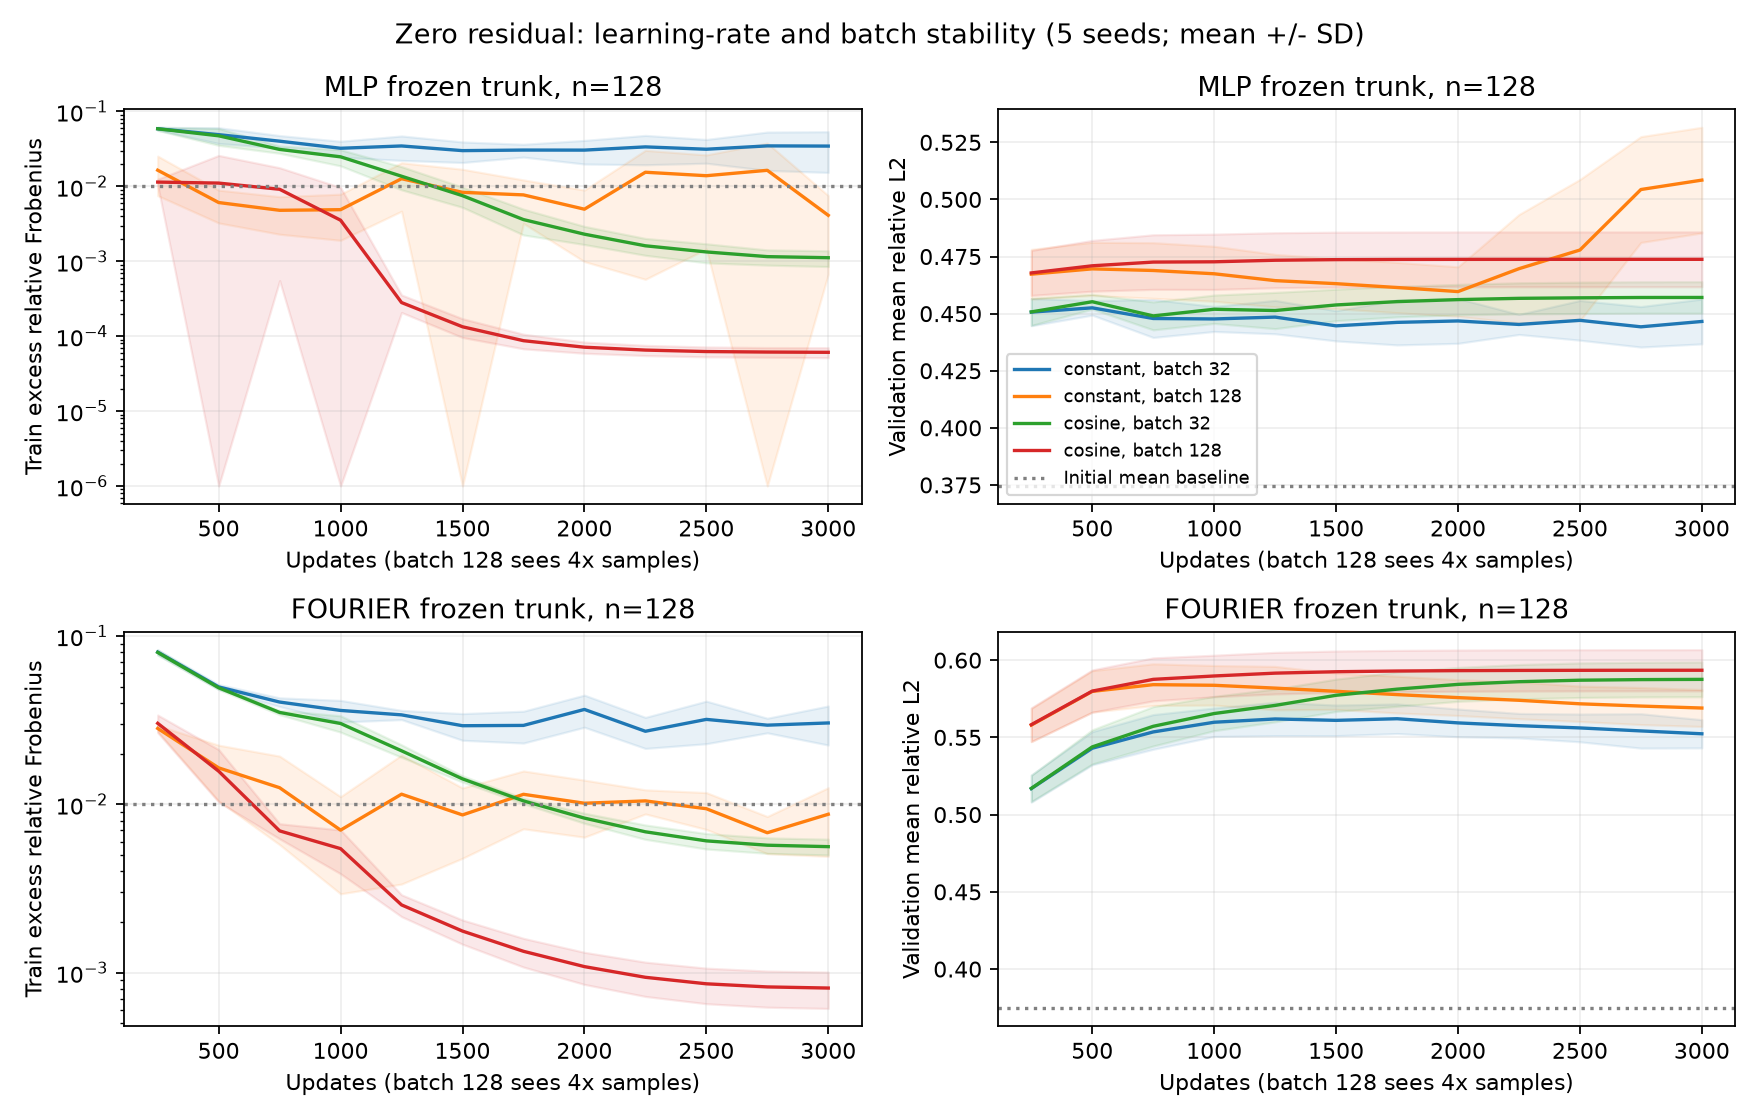
\includegraphics[width=.98\linewidth]{../results/public_stability_v1/stability_curves.png}
\caption{Training fit and validation behavior. Shading is seed standard deviation,
not a confidence interval over independent datasets. Equal updates are not equal compute.}
\end{figure}

\section{Limitations and conclusion}
This is one public PDE, coefficient, time and split. Later families use validation
only, and early test results are exploratory. Reused trunks, weak initial baselines,
rank sensitivity and unequal sample exposure limit generalization of the conclusions.
The projection identity, zero initialization and cosine scheduling are not new methods.
The contribution candidate is an auditable diagnostic intervention sequence.
Training-only POD and faithful two-step references, data scaling, a second PDE and
fresh-holdout confirmation remain necessary.

Historical claims of pure optimization attribution, universal variance floors and
confirmed alignment mechanisms are withdrawn. A small supervised value error does
not guarantee a small PDE residual. Sampler correctness instead requires explicit
paired-value and shape contracts. Full historical drafts remain archived.

\paragraph{Reproducibility and status.}
Eighteen software tests passed after manuscript revision, including manuscript checks;
CPU/CUDA resume
checks. Checkpoints preserve model, optimizer, random state and schedule position.
This is a local research draft, not a completed anonymized release or submitted paper.
AI assistance was used for code and writing; the numerical evidence comes from
executed scripts. The full Markdown manuscript is the authoritative detailed text.

\begin{thebibliography}{7}
\bibitem{lee2023} S. Lee and Y. Shin.
On the training and generalization of deep operator networks.
\url{https://arxiv.org/abs/2309.01020}, 2023.
\bibitem{williams2024} E. Williams, A. Howard, B. Meuris and P. Stinis.
What do physics-informed DeepONets learn? Understanding and improving training
for scientific computing applications. \url{https://arxiv.org/abs/2411.18459}, 2024.
\bibitem{lu2022} L. Lu et al.
A comprehensive and fair comparison of two neural operators (with practical extensions)
based on FAIR data. \url{https://arxiv.org/abs/2111.05512};
journal DOI \url{https://doi.org/10.1016/j.cma.2022.114778}.
\bibitem{pdebench} M. Takamoto et al.
PDEBench: An Extensive Benchmark for Scientific Machine Learning.
NeurIPS Datasets and Benchmarks, 2022. \url{https://arxiv.org/abs/2210.07182}.
\bibitem{rezero} T. Bachlechner et al.
ReZero is all you need: fast convergence at large depth.
PMLR 161, 2021. \url{https://proceedings.mlr.press/v161/bachlechner21a.html}.
\bibitem{sgdr} I. Loshchilov and F. Hutter.
SGDR: Stochastic Gradient Descent with Warm Restarts.
ICLR 2017. \url{https://arxiv.org/abs/1608.03983}.
\bibitem{keskar} N. S. Keskar et al.
On Large-Batch Training for Deep Learning: Generalization Gap and Sharp Minima.
ICLR 2017. \url{https://arxiv.org/abs/1609.04836}.
\end{thebibliography}
\end{document}
